\begin{flushright} {\tiny {\color{gray} python\_codes/fieldstone\_130/text.tex}} \end{flushright}

%\lstinputlisting[language=bash,basicstyle=\small]{python_codes/fieldstone_130/keywords}

\begin{center}
\fbox{\textbf{\huge \color{teal} P}}
Codes at \url{https://github.com/cedrict/fieldstone/tree/master/python_codes/fieldstone_130}
\end{center}

\par\noindent\rule{\textwidth}{0.4pt}

%%%%%%%%%%%%%%%%%%%%%%%%%%%%%%%%%%%%%%%%%%%%%%%%%%%%%%%%%%%%%%%%%%%%%%%%%%%%%%%%%%%%%%%%%%%%%%

This is based on Simpson's book \cite{simp17}, chapter 7.3.

As an introduction to the topic of how the FEM can be
performed on systems of equations, we consider the following equations
\begin{eqnarray}
\frac{\partial A}{\partial t} &=& \Delta A  + \gamma (a-A+A^2B) \\
\frac{\partial B}{\partial t} &=& d \Delta B  + \gamma (b-A^2B) 
\end{eqnarray}
with the two unknowns, $A$ and $B$. This system of equations is used to model the interaction between
two interacting chemicals $A$ and $B$.

$B$ represents the concentration of
a ``substrate'' (inhibitor) chemical that is consumed in a reaction by some chemical ``activator'',
with concentration $A$. The reaction produces the activator, which explains the $A^2B$ terms in both
equations. Both substances are also produced at some background rate ($\gamma a$ for $A$ and $\gamma b$ for $B$,
respectively) and $A$ decays with first-order kinetics at a rate $\gamma$.

This ``substrate depletion'' reaction
model is known as Schnakenberg kinetics. This
model is most widely applied in biology, but it might also be relevant in Earth science to explain
the formation of self-organizing patterns, for example, related to mineral growth, stromatolites and
corals, concretions, and so on.

\begin{center}
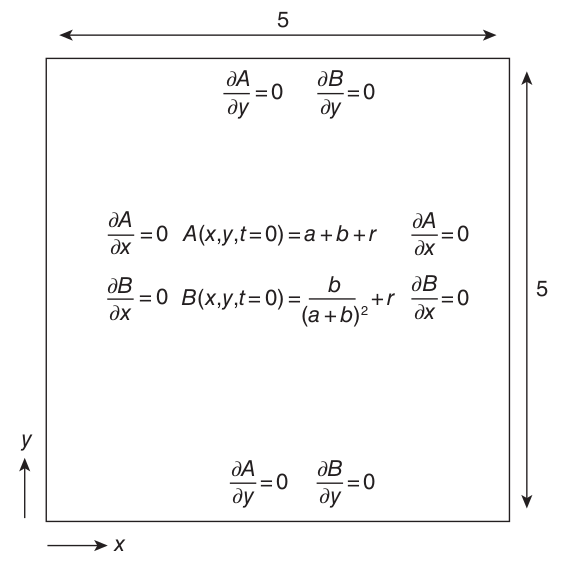
\includegraphics[width=5cm]{python_codes/fieldstone_130/images/simpson1}
\end{center}

The domain is a square of size 5. At $t=0$ the fields are given by
\begin{eqnarray}
A(x,y)&=&a+b+r \nn\\
B(x,y)&=& \frac{b}{(a+b)^2} +r
\end{eqnarray}
which is the steady-state solution with a small random perturbation $r$ (that has a maximum amplitude
of 1/100). No flux (zero gradient) conditions are considered across all lateral boundaries.

In the book we find: 
\begin{verbatim}
lx = 5 ; % length of x domain
ly = 5 ; % length of y domain
d = 20 ; % diffusivity of species B
a = 0.05 ; % growth rate of species A
b = 1 ; % growth rate of species B
gamma = 600 ; % kinetics
amp = 0.01 ; % max. amplitude of random noise
ntime = 200 ; % total number of time steps to compute
nxe = 50 ; % number of elements in x-direction
nye = 50 ; % number of elements in y-direction
dt = 5e-4 ; % time step
\end{verbatim}


\begin{center}
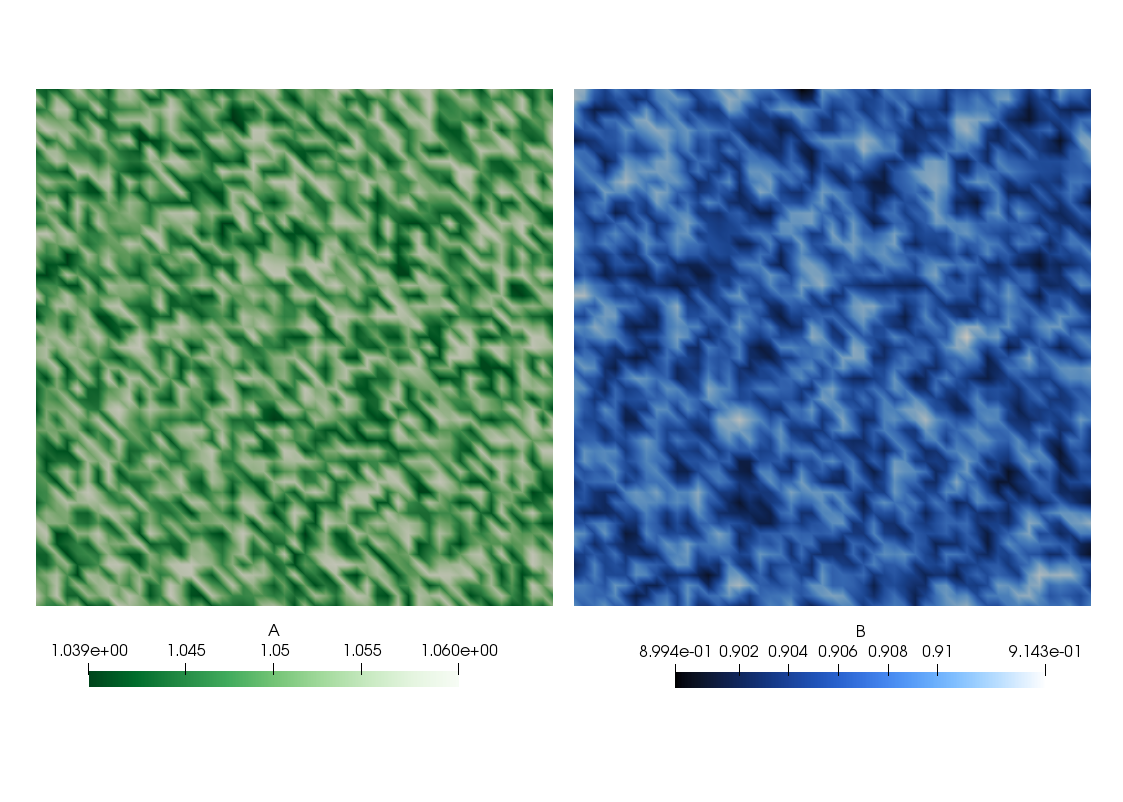
\includegraphics[width=10cm]{python_codes/fieldstone_130/results/AB_000}
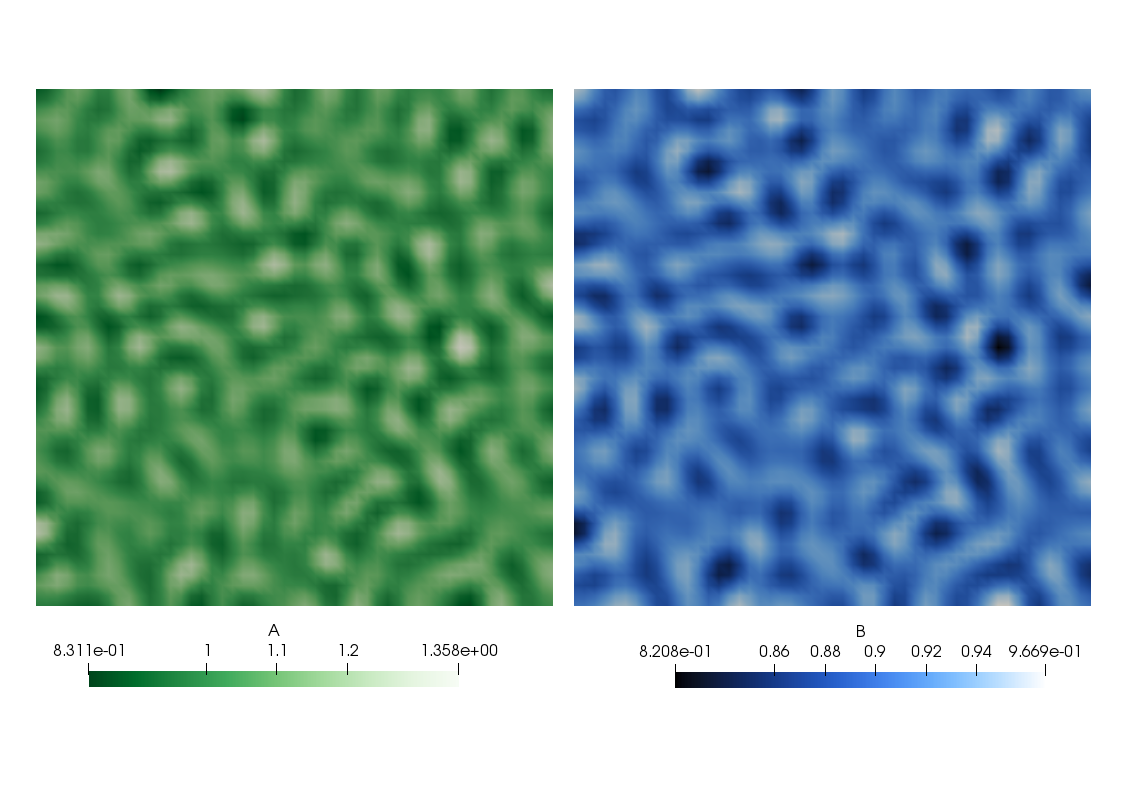
\includegraphics[width=10cm]{python_codes/fieldstone_130/results/AB_200}
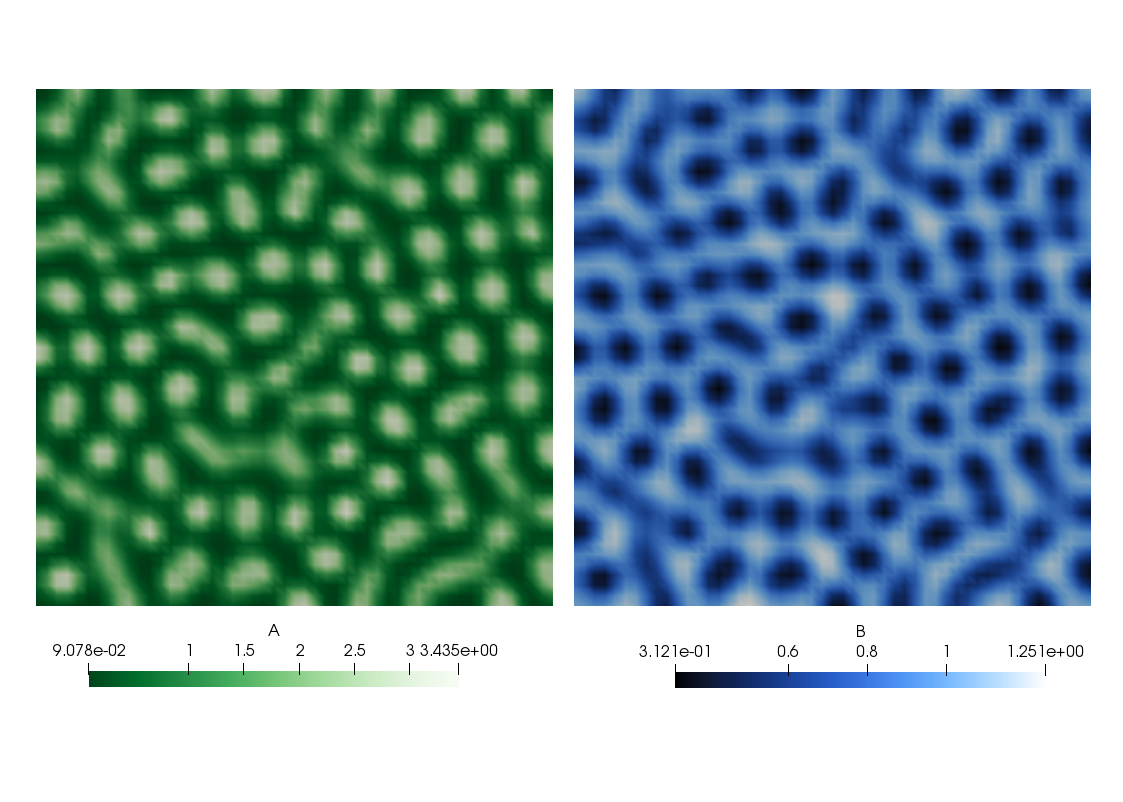
\includegraphics[width=10cm]{python_codes/fieldstone_130/results/AB_400}
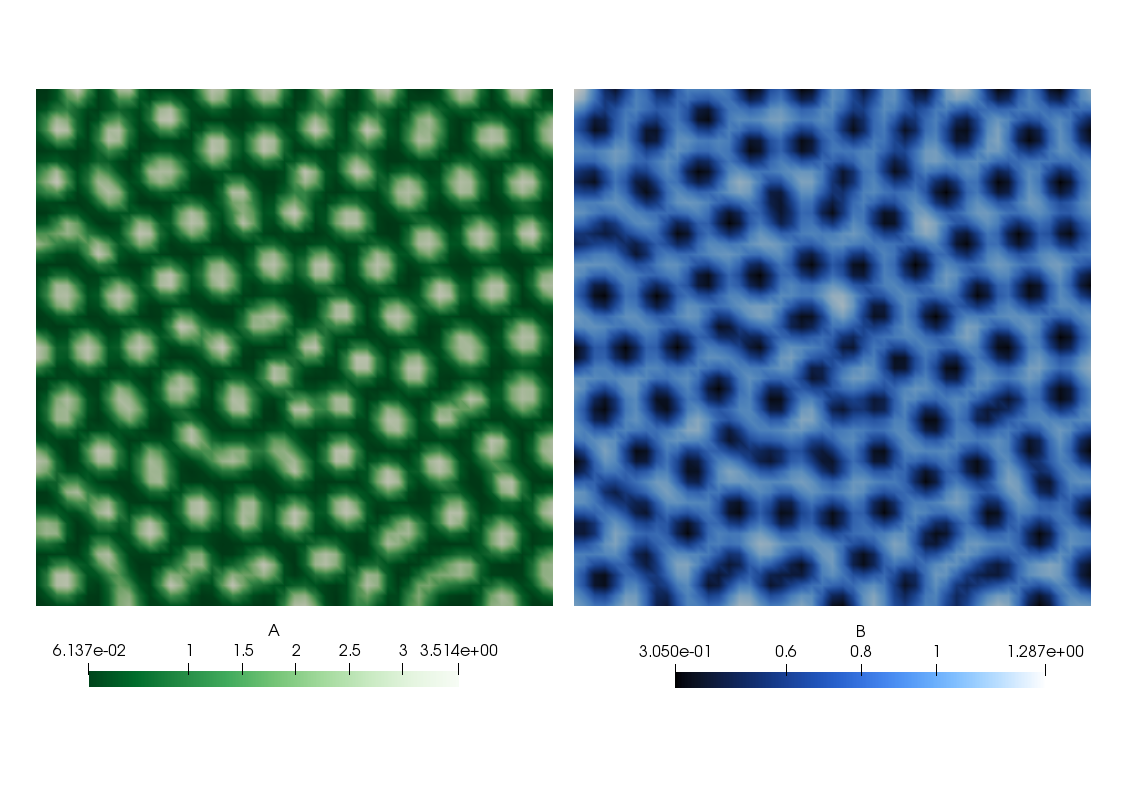
\includegraphics[width=10cm]{python_codes/fieldstone_130/results/AB_600}
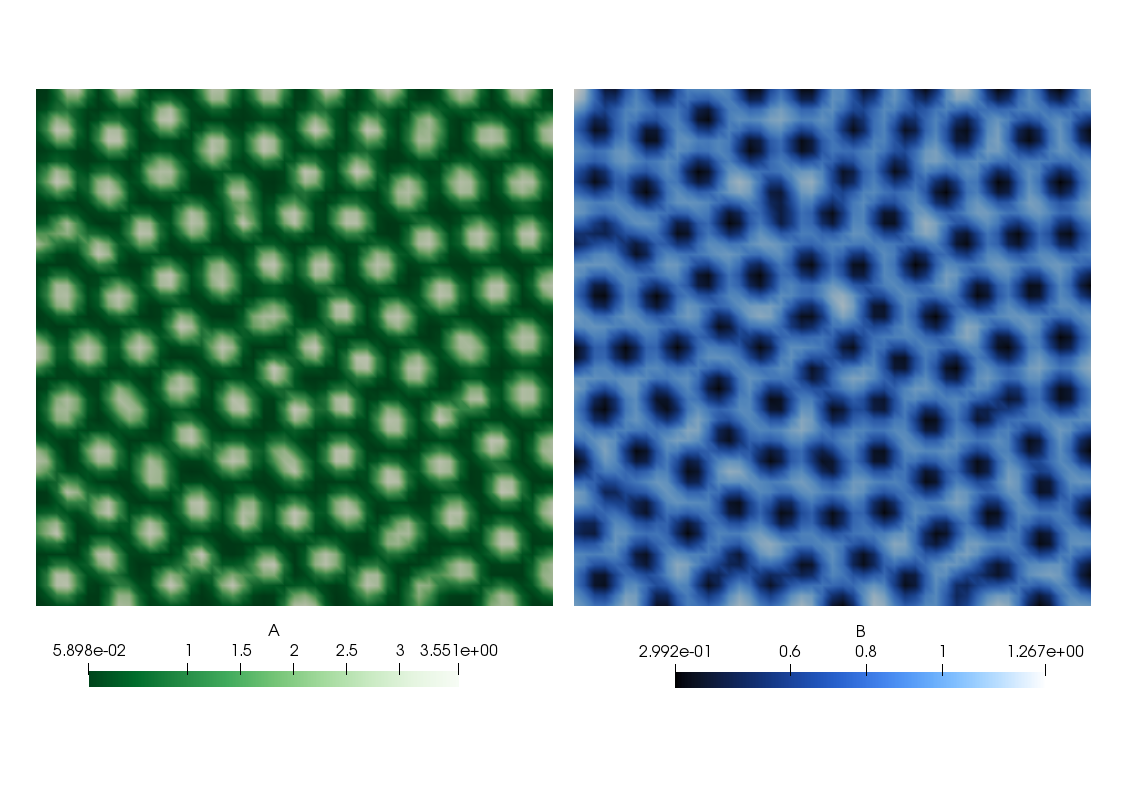
\includegraphics[width=10cm]{python_codes/fieldstone_130/results/AB_800}\\
{\captionfont phases $A$ and $B$ at time steps 0,200,400,600,800.}
\end{center}


This is a rough take.
I need nonlinear iterations to take care of the nonlinearities introduced by the rhs
I need to explaore whether part of the rhs could not make its way in the matrix. 
Quid of the nl convergence ?
Also need to document of the global matrix is partitioned and assembled.
write about weak forms of PDEs.
Plot statistics. What about steady state ?
This is 1st order implicit in time. Crank-Nicolson ?
Include refs of the book. 
